\chapter{Câu hỏi ôn tập}
\ANSMCQ{
	\begin{center}
		\begin{tabular}{|m{2.8em}|m{2.8em}|m{2.8em}|m{2.8em}|m{2.8em}|m{2.8em}|m{2.8em}|m{2.8em}|m{2.8em}|m{2.8em}|}
			\hline
			1B & 2B & 3B & 4A & 5D & 6C & 7A & 8C & 9C & 10D\\
			\hline
			11C & 12B & 13C & 14C & 15D & 16B  & 17A & 18C & 19C & 20D\\
			\hline
			21B & 22C & 23A & 24C & 25C &  &  &  &  & \\
			\hline
		\end{tabular}
\end{center}}
\begin{enumerate}[label=\bfseries Câu \arabic*:]
	\item Một sóng cơ với tần số $f$ truyền trên một sợi dây đàn hồi vơi tốc độ $v$ và có bước sóng $\lambda$. Hệ thức đúng là
	\begin{mcq}(4)
		\item $v=\dfrac{\lambda}{f}$.
		\item $v=\lambda f$.
		\item $v=2\pi\lambda f$.
		\item $v=\dfrac{f}{\lambda}$.
	\end{mcq}
\hideall{
\textbf{Đáp án B.}
}	

\item Sóng điện từ
\begin{mcq}
	\item là sóng dọc và truyền được trong chân không.
	\item là sóng ngang và truyền được trong chân không.
	\item là sóng dọc và không truyền được trong chân không.
	\item là sóng ngang và không truyền được trong chân không.
\end{mcq}
	
	\hideall{
\textbf{Đáp án B.}\\	
Sóng điện từ là sóng ngang và truyền được trong chân không.
}

\item Xét các tia gồm tia hồng ngoại, tia X, tia gamma, tia $\beta.$ Tia có bản chất khác với các tia còn lại là
\begin{mcq}(4)
	\item tia gamma.
	\item tia $\beta$.
	\item tia X.
	\item tia hồng ngoại.
\end{mcq}
\hideall{
\textbf{Đáp án B.}\\
 Tia $\beta$ không có bản chất là sóng điện từ.
}

\item Mặt đèn hình của ti vi sử dụng ống phóng điện tử thường được chế tạo rất dày là nhằm mục đích 
\begin{mcq}(2)
	\item chặn các tia rơnghen thoát ra ngoài.
	\item giảm độ nóng cho mặt đèn hình.
	\item tăng độ bền cơ học cho đèn hình.
	\item ngăn không cho các electron thoát ra ngoài.
\end{mcq}
\hideall{
\textbf{Đáp án A.}
}

\item Một sóng cơ hình sin truyền theo trục $Ox$. Phương trình dao động của một phần tử môi trường trên $Ox$ là $u=\xsi{2\cos10t}{\milli\meter}$. Biên độ của sóng là
\begin{mcq}(4)
	\item $\SI{10}{\milli\meter}$.
	\item $\SI{4}{\milli\meter}$.
	\item $\SI{5}{\milli\meter}$.
	\item $\SI{2}{\milli\meter}$.
\end{mcq}
\hideall{
\textbf{Đáp án D.}
}

\item Khi nói về tia X, phát biều nào sau đây đúng?
\begin{mcq}(2)
	\item Tia X là dòng hạt mang điện.
	\item Tia X không có khả năng đâm xuyên.
	\item Tia X có bản chất là sóng điện từ.
	\item Tia X không truyền được trong chân không.
\end{mcq}
\hideall{
\textbf{Đáp án C.}
}

\item Phát biểu nào sau đây \textbf{không đúng} với sóng cơ?
\begin{mcq}
	\item Sóng cơ có thể lan truyền được trong môi trường chân không.
	\item Sóng cơ có thể lan truyền được trong môi trường chất lỏng.
	\item Sóng cơ có thể lan truyền được trong môi trường chất khí.
	\item Sóng cơ có thể lan truyền được trong môi trường chất rắn.
\end{mcq}
\hideall{
\textbf{Đáp án A.}\\
Sóng cơ không truyền được trong chân không.
}

\item Trên mặt nước đủ rộng có một nguồn điểm O dao động điều hòa theo phương thẳng đứng tạo ra một hệ sóng tròn đồng tâm O lan tỏa ra xung quanh. Thả một nút chai nhỏ nổi trên mặt nước nơi có sóng truyền qua thì nút chai 
\begin{mcq}(2)
	\item sẽ bị sóng cuốn ra xa nguồn.
	\item sẽ dịch chuyển lại gần nguồn.
	\item sẽ dao động tại chỗ theo phương thẳng đứng.
	\item sẽ dao động theo phương nằm ngang.
\end{mcq}
\hideall{
\textbf{Đáp án C.}
}

\item Trong hiện tượng sóng dừng trên dây đàn hồi, khoảng cách giữa hai nút sóng liên tiếp bằng
\begin{mcq}(2)
	\item hai lần bước sóng.
	\item một bước sóng.
	\item một nửa bước sóng.
	\item một phần tư bước sóng.
\end{mcq}
\hideall{
\textbf{Đáp án C.}\\
Khoảng cách giữa hai nút sóng liên tiếp bằng một nửa bước sóng.
}

\item Âm mà tai người nghe được có tần số $f$ nằm trong khoảng 
\begin{mcq}(2)
	\item $\SI{16}{\kilo\hertz}\le f\le \SI{20000}{\hertz}$.
	\item $\SI{16}{\hertz}\le f\le \SI{30000}{\hertz}$.
	\item $f\ge \SI{20000}{\hertz}$.
	\item $\SI{16}{\hertz}\le f\le \SI{20}{\kilo\hertz}$.
\end{mcq}
\hideall{
\textbf{Đáp án D.}\\
Tai người nghe được âm có tần số trong khoảng từ $\SI{16}{\hertz}$ đến $\SI{20000}{\hertz}$.
}

\item Trên một sợi dây đang có sóng dừng. Biết sóng truyền trên dây có bước sóng $\SI{30}{\centi\meter}$. Khoảng cách ngắn nhất từ một nút đến một bụng là 
\begin{mcq}(4)
	\item $\SI{15}{\centi\meter}$.
	\item $\SI{30}{\centi\meter}$.
	\item $\SI{7.5}{\centi\meter}$.
	\item $\SI{60}{\centi\meter}$.
\end{mcq}
\hideall{
\textbf{Đáp án C.}\\
Khoảng cách ngắn nhất từ một nút đến một bụng là $d_\text{min}=\dfrac{\lambda}{4}=\SI{7.5}{\centi\meter}$.
}

\item Một bức xạ đơn sắc có tần số $\SI{3E14}{\hertz}$. Lấy $c=\SI{3E8}{\meter/\second}$. Đây là 
\begin{mcq}(2)
	\item bức xạ tử ngoại.
	\item bức xạ hồng ngoại.
	\item ánh sáng đỏ.
	\item ánh sáng tím.
\end{mcq}
\hideall{
\textbf{Đáp án B.}\\
$$\lambda=\dfrac{c}{f}=\SI{E-6}{\meter}\rightarrow \text{bức xạ thuộc vùng hồng ngoại.}$$
}


\item Phát biểu nào sau đây là \textbf{sai} khi nói về sóng điện từ?
\begin{mcq}
	\item Sóng điện từ là sóng ngang.
	\item Khi sóng điện từ lan truyền, vectơ cường độ điện trường luôn vuông góc với vectơ cảm ứng từ.
	\item Khi sóng điện từ lan truyền, vectơ cường độ điện trường luôn cùng phương với vectơ cảm ứng từ.
	\item Sóng điện từ lan truyền được trong chân không.
\end{mcq}
\hideall{
\textbf{Đáp án C.}\\
 Khi sóng điện từ lan truyền, vector cường độ điện trường có phương vuông góc với vector cảm ứng từ.
}

\item Tiến hành thí nghiệm Young về giao thoa ánh sáng với ánh sáng đơn sắc có bước sóng $\SI{0.6}{\micro\meter}$. Khoảng cách giữa hai khe là $\SI{0.3}{\milli\meter}$, khoảng cách từ mặt phẳng chứa hai khe đến màn quan sát là $\SI{2}{\meter}$. Trên màn, khoảng cách giữa vân sáng bậc 3 và vân sáng bậc 5 ở hai phía so với vân sáng trung tâm là
\begin{mcq}(4)
	\item $\SI{12}{\milli\meter}$.
	\item $\SI{8}{\milli\meter}$.
	\item $\SI{32}{\milli\meter}$.
	\item $\SI{20}{\milli\meter}$.
\end{mcq} 
\hideall{
\textbf{Đáp án C.}\\
$$\Delta x=8\dfrac{\lambda D}{a}=\SI{32}{\milli\meter}.$$
}

\item Một sợi dây đàn hồi dài $\SI{60}{\centi\meter}$, được rung với tần số $\SI{50}{\hertz}$, trên dây tạo thành một sóng dừng ổn định với 4 bụng sóng, hai đầu là hai nút sóng. Tốc độ truyền sóng trên dây là
\begin{mcq}(4)
	\item $\SI{60}{\centi\meter/\second}$.
	\item $\SI{75}{\centi\meter/\second}$.
	\item $\SI{12}{\centi\meter/\second}$.
	\item $\SI{15}{\centi\meter/\second}$.
\end{mcq}
\hideall{
\textbf{Đáp án D.}\\
$$\ell=k\cdot\dfrac{v}{2f}\Rightarrow v=\dfrac{2\ell f}{k}=\SI{15}{\meter/\second}.$$
}

\item  Trong bài thực hành xác định tốc độ truyền âm, một học sinh đo được bước sóng của âm là $\lambda=\xsi{\left(77,0\pm0,5\right)}{\centi\meter}$. Biết tần số nguồn âm là $f=\xsi{\left(440\pm 10\right)}{\hertz}$. Tốc độ truyền âm mà học sinh này đo được trong thí nghiệm là
\begin{mcq}(2)
	\item $\xsi{\left(338\pm 9\right)}{\meter/\second}$.
	\item $\xsi{\left(339\pm 10\right)}{\meter/\second}$.
	\item $\xsi{\left(339\pm 9\right)}{\meter/\second}$.
	\item $\xsi{\left(338\pm 10\right)}{\meter/\second}$.
\end{mcq}
\hideall{
\textbf{Đáp án B.}\\
Tốc độ truyền âm: $\overline{v}=\overline{\lambda}\cdot\overline{f}\approx\SI{339}{\meter/\second}.$\\
Sai số:
$$\dfrac{\Delta v}{\overline{v}}=\dfrac{\Delta \lambda}{\overline{\lambda}}+\dfrac{\Delta f}{\overline{f}}\Rightarrow \Delta v\approx\SI{10}{\meter/\second}.$$
}

\item Trong thí nghiệm giao thoa sóng trên mặt nước, hai nguồn AB cách nhau $\SI{11}{\centi\meter}$ dao động cùng pha cùng tần số $\SI{20}{\hertz}$, tốc độ truyền sóng trên mặt nước $\SI{80}{\centi\meter/\second}$. Số đường dao động cực đại và cực tiểu quan sát được trên mặt nước là
\begin{mcq}(2)
	\item 5 cực đại và 6 cực tiểu.
	\item 4 cực đại và 5 cực tiểu.
	\item 6 cực đại và 5 cực tiểu.
	\item 5 cực đại và 4 cực tiểu.
\end{mcq}
\hideall{
\textbf{Đáp án A.}
}

\item Thực hiện thí nghiệm sóng dừng trên một sợi dây thẳng đứng có đầu trên cố định, đầu dưới gắn với cần rung dao động theo phương ngang với tần số $\SI{10}{\hertz}$. Quan sát trên dây thấy có 4 bó sóng và đo được khoảng cách hai đầu dây là $\SI{0.8}{\meter}$. Tốc độ truyền sóng trên dây là
\begin{mcq}(4)
	\item $\SI{2}{\meter/\second}$.
	\item $\SI{8}{\meter/\second}$.
	\item $\SI{4}{\meter/\second}$.
	\item $\SI{16}{\meter/\second}$.
\end{mcq}
\hideall{
\textbf{Đáp án C.}
}

\item Một sóng cơ lan truyền trong một môi trường đồng chất, đẳng hướng với tần số $\SI{20}{\hertz}$. Tốc độ truyền sóng trong môi trường là$\SI{25}{\centi\meter/\second}$. Bước sóng là
\begin{mcq}(4)
	\item $\SI{0.8}{\centi\meter}$.
	\item $\SI{5.0}{\meter}$.
	\item $\SI{1.25}{\centi\meter}$.
	\item $\SI{5.0}{\centi\meter}$.
\end{mcq}
\hideall{
\textbf{Đáp án C.}
}

\item Trong thí nghiệm Young về giao thoa ánh sáng, khoảng cách giữa hai khe là $a=\SI{1}{\milli\meter}$, khoảng cách từ hai khe đến màn là $D=\SI{2.5}{\meter}$. Nguồn S phát ra ánh sáng trắng có bước sóng từ $\SI{380}{\nano\meter}$ đến $\SI{760}{\nano\meter}$. Vùng phủ nhau của quang phổ bậc 3 và quang phổ bậc 4 có bề rộng là
\begin{mcq}(4)
\item $\SI{0.76}{\milli\meter}$.
\item $\SI{1.14}{\milli\meter}$.
\item $\SI{1.52}{\milli\meter}$.
\item $\SI{1.9}{\milli\meter}$.
\end{mcq}
\hideall{
\textbf{Đáp án D.}\\
$$\Delta x=x_\text{3đ}-x_\text{4t}=\SI{1.9}{\milli\meter}.$$
}

\item Sóng dừng hình thành trên một sợi dây, khi xảy ra ổn định hình ảnh của sợi dây có dạng như hình vẽ. Biết chiều dài của sợi dây là $\ell $ sóng truyền trên dây với bước sóng $\lambda.$ Kết luận nào sau đây là đúng?
\begin{center}
	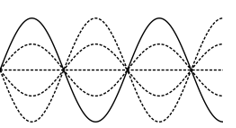
\includegraphics[width=0.3\linewidth]{../figs/Y23-VN11-PH-C2-Q-1}
\end{center}
\begin{mcq}(4)
	\item $\lambda=3\ell$.
	\item $\lambda=\dfrac{7\ell}{4}$.
	\item $\lambda=2\ell$.
	\item $\lambda=\dfrac{\ell}{2}$.
\end{mcq}
\hideall{
\textbf{Đáp án B.}
}

\item Một sóng truyền theo phương AB. Tại một thời điểm nào đó, hình dạng sóng có dạng như hình vẽ. Biết rằng điểm M đang đi lên vị trí cân bằng. Khi đó điểm N đang chuyển động
\begin{center}
	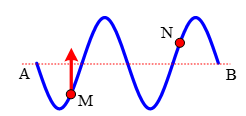
\includegraphics[width=0.3\linewidth]{../figs/Y23-VN11-PH-C2-Q-2}
\end{center}
\begin{mcq}(4)
	\item chạy ngang.
	\item đi xuống.
	\item đi lên
	\item đứng yên
\end{mcq}
\hideall{
\textbf{Đáp án C.}
}

\item Xét một sợi dây đàn hồi, có một đầu cố định, một đầu tự do. Với tần số $\SI{24}{\hertz}$ thì trên dây có sóng dừng. Theo lí thuyết sóng dừng, trong các tần số $f_1=\SI{16}{\hertz}$, $f_2=\SI{36}{\hertz}$, $f_3=\SI{48}{\hertz}$, $f_4=\SI{56}{\hertz}$, $f_5=\SI{80}{\hertz}$, $f_6=\SI{96}{\hertz}$ thì số tần số có thể tạo được sóng dừng trên dây là
\begin{mcq}(4)
	\item 1.
	\item 2.
	\item 6.
	\item 5.
\end{mcq}
\hideall{
\textbf{Đáp án A.}\\
Sóng dừng trên dây 1 đầu cố định và 1 đầu tự do thì tần số của nguồn phải thoả: $f_m=mf_1$ với $f_1=\dfrac{v}{4\ell}$ là tần số cơ bản, $m$ là các số lẻ.\\
Như vậy $\dfrac{f_n}{f_m}=\dfrac{n}{m}$ với $n, m$ là các số lẻ.\\
$\rightarrow$ chỉ có $f_5$ thoả mãn.
}

\item Trong thí nghiệm về dao thoa sóng trên mặt nước, hai nguồn kết hợp A, B dao động với tần số $f=\SI{16}{\hertz}$ và cùng pha. Tại điểm M cách các nguồn lần lượt là $d_1=\SI{30}{\centi\meter}$, $d_2=\SI{25.5}{\centi\meter}$, sóng có biên độ cực đại. Giữa M và đường trung trực AB có hai dãy cực đại khác. Tốc độ truyền sóng trên mặt nước là
\begin{mcq}(4)
	\item $\SI{12}{\centi\meter/\second}$.
	\item $\SI{26}{\centi\meter/\second}$.
	\item $\SI{24}{\centi\meter/\second}$.
	\item $\SI{20}{\centi\meter/\second}$.
\end{mcq}
\hideall{
\textbf{Đáp án C.}\\
M nằm trên dãy cực đại thứ 3:
$$\lambda=\dfrac{d_1-d_2}{3}=\SI{1.5}{\centi\meter}\Rightarrow v=\lambda f=\SI{24}{\centi\meter/\second}.$$
}

\item Thí nghiệm giao thoa Young với ánh sáng đơn sắc có bước sóng $\lambda$, khoảng cách giữa hai khe $a=\SI{1}{\milli\meter}$. Ban đầu, tại M cách vân trung tâm $\SI{5.25}{\milli\meter}$ người ta quan sát được vân sáng bậc 5. Giữ cố định màn chứa hai khe, di chuyển từ từ màn quan sát ra xa và dọc theo đường thẳng vuông góc với mặt phẳng chứa hai khe một đoạn $\SI{0.75}{\meter}$ thì thấy tại M chuyển thành vân tối lần thứ hai. Bước sóng $\lambda$ có giá trị là
\begin{mcq}(4)
	\item $\SI{0.64}{\micro\meter}$.
	\item $\SI{0.70}{\micro\meter}$.
	\item $\SI{0.60}{\micro\meter}$.
	\item $\SI{0.50}{\micro\meter}$.
\end{mcq}
\hideall{
\textbf{Đáp án C.}\\
Ta có:
$$\begin{cases}
	x_M=5\dfrac{\lambda D}{a}\\
	x_M=3,5\dfrac{\left(D+0,75\right)\lambda}{a}
\end{cases}
\Rightarrow D=\SI{1.75}{\meter}.$$
Bước sóng ánh sáng dùng trong thí nghiệm:
$$\lambda=\dfrac{x_M a}{5D}=\SI{0.6}{\micro\meter}.$$
}

\end{enumerate}